\documentclass{article}
\usepackage{graphicx}
\usepackage{fancyhdr}
\usepackage{extramarks}
\usepackage{amsmath}
\usepackage{amsthm}
\usepackage{amsfonts}
\usepackage{tikz}
\usepackage[plain]{algorithm}
\usepackage{algpseudocode}
\usepackage{enumerate}
\usepackage{tikz}
\usepackage{xifthen}
\usepackage{xparse}
\usepackage{listings}
\usepackage{amsmath, amssymb}
\usepackage{subfigure}
\usepackage{lipsum}

\usetikzlibrary{automata,positioning}

%
% Basic Document Settings
%  

\topmargin=-0.45in
\evensidemargin=0in
\oddsidemargin=0in
\textwidth=6.5in
\textheight=9.0in
\headsep=0.25in

\linespread{1.1}

\pagestyle{fancy}
\lhead{\hmwkAuthorName}
\chead{\hmwkClass : \hmwkTitle}
\rhead{\firstxmark}
\lfoot{\lastxmark}
\cfoot{\thepage}

\renewcommand\headrulewidth{0.4pt}
\renewcommand\footrulewidth{0.4pt}

\setlength\parindent{0pt}

%
% Create Problem Sections
%

\newcommand{\enterProblemHeader}[1]{
    \nobreak\extramarks{}{Problem \arabic{#1} continued on next page\ldots}\nobreak{}
    \nobreak\extramarks{Problem \arabic{#1} (continued)}{Problem \arabic{#1} continued on next page\ldots}\nobreak{}
}

\newcommand{\exitProblemHeader}[1]{
    \nobreak\extramarks{Problem \arabic{#1} (continued)}{Problem \arabic{#1} continued on next page\ldots}\nobreak{}
    \stepcounter{#1}
    \nobreak\extramarks{Problem \arabic{#1}}{}\nobreak{}
}

\newcommand*\circled[1]{\tikz[baseline=(char.base)]{
		\node[shape=circle,draw,inner sep=2pt] (char) {#1};}}


\setcounter{secnumdepth}{0}
\newcounter{partCounter}
\newcounter{homeworkProblemCounter}
\setcounter{homeworkProblemCounter}{1}
\nobreak\extramarks{Problem \arabic{homeworkProblemCounter}}{}\nobreak{}

%
% Homework Problem Environment
%
% This environment takes an optional argument. When given, it will adjust the
% problem counter. This is useful for when the problems given for your
% assignment aren't sequential. See the last 3 problems of this template for an
% example.
%

\newenvironment{homeworkProblem}[1][-1]{
    \ifnum#1>0
        \setcounter{homeworkProblemCounter}{#1}
    \fi
    \section{Problem \arabic{homeworkProblemCounter}}
    \setcounter{partCounter}{1}
    \enterProblemHeader{homeworkProblemCounter}
}{
    \exitProblemHeader{homeworkProblemCounter}
}

%
% Homework Details
%   - Title
%   - Class
%   - Due date
%   - Name
%   - Student ID

\newcommand{\hmwkTitle}{Homework\ \#12}
\newcommand{\hmwkClass}{Probability \& Statistics for EECS}
\newcommand{\hmwkDueDate}{May 07, 2023}
\newcommand{\hmwkAuthorName}{Wang Yunfei}
\newcommand{\hmwkAuthorID}{2021533135}


%
% Title Page
%

\title{
    \vspace{2in}
    \textmd{\textbf{\hmwkClass:\\  \hmwkTitle}}\\
    \normalsize\vspace{0.1in}\small{Due\ on\ \hmwkDueDate\ at 23:59}\\
	\vspace{4in}
}

\author{
	Name: \textbf{\hmwkAuthorName} \\
	Student ID: \hmwkAuthorID}
\date{}

\renewcommand{\part}[1]{\textbf{\large Part \Alph{partCounter}}\stepcounter{partCounter}\\}

%
% Various Helper Commands
%

% Useful for algorithms
\newcommand{\alg}[1]{\textsc{\bfseries \footnotesize #1}}
% For derivatives
\newcommand{\deriv}[1]{\frac{\mathrm{d}}{\mathrm{d}x} (#1)}
% For partial derivatives
\newcommand{\pderiv}[2]{\frac{\partial}{\partial #1} (#2)}
% Integral dx
\newcommand{\dx}{\mathrm{d}x}
% Alias for the Solution section header
\newcommand{\solution}{\textbf{\large Solution}}
% Probability commands: Expectation, Variance, Covariance, Bias
\newcommand{\E}{\mathrm{E}}
\newcommand{\Var}{\mathrm{Var}}
\newcommand{\Cov}{\mathrm{Cov}}
\newcommand{\Bias}{\mathrm{Bias}}

\begin{document}

\maketitle

\pagebreak

\begin{homeworkProblem}[1]
\solution
\begin{enumerate}[(a)]
    \item 
    First p is given a $Unif(0,1)$, then we can model it as a r.v.$\in [0,1]$. Therefore, the prior distribution $p\sim Beta(1,1)$.\\
    Second we can use Beta-Binomial Conjugacy which we have proved in class so that we can intuitively explain the process with the chain rule of bayes rule.\\
    At the begining, depending on the data $X_1=x_1$, we can update the prior distribution and get a middle distribution $Beta(1+x_1,1+(1-x1))$. And then we can seem this as a new prior distribution and update it untill using every data we have.\\
    So finally, we can get the posterior distribution $p|X_1=x_1,\cdots,X_n=x_n\sim Beta(1+x_1+x_2+\cdots+x_n,n+1-(x_1+x_2+\cdots+x_n))$.\\
    Therefore, from the posterior distribution, we can prove that we just need one-dimensional quantity $x_1+x_2+\cdots+x_n$ to obtain the posterior distribution.
\end{enumerate}
\begin{enumerate}[(b)]
    \item 
    For this question we can use LOTP to solve it,
    \begin{align*}
        P(X_{n+1}|X_1+X_2+\cdots+X_n=k)&=\int_{0}^{1} P(X_{n+1}|X_1+X_2+\cdots+X_n=k,p)f(p|X_1+X_2+\cdots+X_n) \,dp\\
        &=\frac{\Gamma (n+2)}{\Gamma (k+1)\Gamma(n+1-k)}\int_{0}^{1}p*p^k(1-p)^{n-k}  \,dp \\
        &=\frac{\Gamma (n+2)}{\Gamma (k+1)\Gamma(n+1-k)}\frac{\Gamma (k+2)\Gamma(n+1-k)}{\Gamma(n+3)}\\
        &=\frac{k+1}{n+2}
    \end{align*}
    Therefore we get it.
\end{enumerate}
\begin{enumerate}[(c)]
    \item
    From we have learned about Beta-Binomial Conjugacy, Laplace's law of succession actually is Bayesian average. We have known the prior distribution $p\sim Unif(0,1)$, and the data model $X_1+X_2+\cdots+X_n$ is a conditional Binomial distribution $Binomial(n,p)$.\\
    Then we can get the posterior distribution when $X_1+X_2+\cdots+X_n=k$, that is $Beta(a+k,b+n-k)$.\\
    And then we can consider about the parameters in posterior distribution. Let $a+k$ is the times of success, and $b+n-k$ is the times of failure.\\
    Then we can predict the condition next day.\\ 
    Then $E[p|X_1+X_2+\cdots+X_n=k]=\frac{a+k}{a+b+n}$, and $a=b=1$.\\
    Therefore $E[p|X_1+X_2+\cdots+X_n=k]=\frac{k+1}{n+2}$, that is the probability that we predict depending on the posterior distribution of the same event happening next day.
\end{enumerate}
\end{homeworkProblem}
\newpage
\begin{homeworkProblem}[2]

\begin{enumerate}[(a)]
    \item
   From the question, we have,
   \begin{align*}
    E[p^2(1-p)^2]&=\int_{0}^{1} p^2(1-p)^2f(p) \,dp \\
    &=\frac{\Gamma(a+b)}{\Gamma(a)\Gamma(b)} \int_{0}^{1} p^2(1-p)^2p^{a-1}(1-p)^{b-1} \,dp \\
    &=\frac{\Gamma(a+b)}{\Gamma(a)\Gamma(b)}\frac{\Gamma(a+2)\Gamma(b+2)}{\Gamma(a+b+4)}\\
    &=\frac{a(a+1)b(b+1)}{(a+b)(a+b+1)(a+b+2)(a+b+3)}
   \end{align*}
\end{enumerate}
\begin{enumerate}[(b)]
    \item
    The posterior distribution for p just depends on the numbers of prior wins and losses for A matter, and not depends on the order.\\
    Because of the coherency of bayes rule, we can always update the prior distribution step by step on the historical data $AAABBAABAB$ so that finally we can get the posterior distribution.\\
    And at the begining, from the question we have $p\sim Beta(1,1)$, and then during the process of updating, when we meet with an A, the first parameter plus one, otherwise, the second parameter plus one.\\
    Then finally, from the prior distribution and the data which is conditionally binomial distribution, we can get the posterior distribution.
\end{enumerate}
\begin{enumerate}[(c)]
    \item
    From the process of (b), we can get the posterior distribution from Beta-Binomial Conjugacy,
    \begin{align*}
        p|AAABBAABAB\sim Beta(7,5)
    \end{align*}
\end{enumerate}
\begin{enumerate}[(d)]
    \item
    These two indicators are conditionally independent but not independent. When given p, the first game and the second game can be seemed as two independent Bernoulli trials. 
    No matter the first game A wins or losses, the result wouldnot have an influence on the second game. But when not given p, if the first game A wins, then like the process of (b), it will facilitate our confidence of A wins, and change our posterior distribution getting in (b).
    Therefore we get it.
\end{enumerate}
\begin{enumerate}[(e)]
    \item
    From the question, we can know A wins two games and loses two games in the first four games. So the probability of this is $\binom{4}{2}p^2(1-p)^2$, when given p.\\
    At the meanwhile, we already have $ p|AAABBAABAB\sim Beta(7,5)$, so we can have,
    \begin{align*}
        &=\binom{4}{2}p^2(1-p)^2\frac{\Gamma(12)}{\Gamma (7)\Gamma(5)}\int_{0}^{1}p^6(1-p)^4  \,dp \\
        &=\binom{4}{2}\frac{\Gamma(12)}{\Gamma (7)\Gamma(5)}\int_{0}^{1}p^8(1-p)^6  \,dp \\
        &=\binom{4}{2}\frac{\Gamma(12)}{\Gamma (7)\Gamma(5)}\frac{\Gamma(9)\Gamma(7)}{\Gamma(16)}\\
        &=\binom{4}{2}\frac{8*7*6*5}{15*14*13*12}\\
        &=\frac{4}{13}
    \end{align*}
\end{enumerate}
\end{homeworkProblem}
\newpage
\begin{homeworkProblem}[3]
\solution
\begin{enumerate}[(a)]
    \item
    Assume n balls to be put in the interval [0,1] randomly, so the distribution of the ball landing in the interval can be regarded as $Unif(0,1)$. \\
    And assume $U_{(1)}=x_1,U_{(2)}=x_2,\cdots U_{(n)}=x_n$, then there are no other balls falling into points except $x_1,x_2,\cdots,x_n$. \\
    And then we can use the story of multinomial to explain this, and get the joint PDF of $U_{(1)},U_{(2)},\cdots U_{(n)}$.\\
    \begin{align*}
        f_{U_{(1)},U_{(2)},\cdots U_{(n)}}=n!
    \end{align*}
\end{enumerate}
\begin{enumerate}[(b)]
    \item
    Assume n balls to be put in the interval [0,1] randomly, so the distribution of the ball landing in the interval can be regarded as $Unif(0,1)$. \\
    And assume $U_{(j)}=x,U_{(k)}=y$, then we can know there are j-1 balls on the left of the point x, and n-k balls on the right of the point y.\\
    Then we can know there are k-j+1 points between point x and point y, including them simultaneously.\\
    Then we can use the story of multinomial to explain this too.\\
    Then we can have the joint PDF of $U_{(j)},U_{(k)}$,
    \begin{align*}
        f_{U_{(j)},U_{(k)}}(x,y)=\frac{n!}{(j-1)!(k-j-1)!(n-k)!}x^{j-1}(y-x)^{k-j-1}(1-y)^{n-k}
    \end{align*}
\end{enumerate}
\begin{enumerate}[(c)]
    \item
    We already have $U_1,\cdots,U_n$ are i.i.d. $Unif(0,1)$. Then we can define a new Bernoulli trial, which means when $U_j<=p$, the trial is thought of a success.\\
    Then Let X mean the number of success, then $X>=j$ means $U_{(j)}<=p$.\\
    Therefore we can have the following formula,
    \begin{align*}
        P(X>=j)&=P(U_{(j)}<=p)\\
        &=\frac{n!}{(j-1)!(n-j)!}(p)^{j-1}(1-p)^{n-j}=\frac{1}{\beta(j,n-j+1)}(p)^{j-1}(1-p)^{n-j}\\
        &=P(B<=p)
    \end{align*}
    Therefore we get it.
\end{enumerate}
\begin{enumerate}[(d)]
    \item
    From what we have proved in (c), let p=x, then we can have $P(X>=j)=P(B<=x)$, and $X\sim Bin(n,x),B\sim Beta(j,n-j+1)$.\\
    So $P(X>=j)=\sum_{k=j}^{n}\binom{n}{k}x^k(1-x)^{n-k}$.\\
    And $P(B<=x)=P(U_{(j)}<=x)=\int_{0}^{x}\frac{n!}{(j-1)!(n-j)!}t^{j-1}(1-t)^{n-j}  \,dt $.\\
    Then $\sum_{k=j}^{n}\binom{n}{k}x^k(1-x)^{n-k}=\int_{0}^{x}\frac{n!}{(j-1)!(n-j)!}t^{j-1}(1-t)^{n-j}\,dt$.
    Therefore we get it.
\end{enumerate}
\end{homeworkProblem}
\newpage
\begin{homeworkProblem}[4]
\solution
\begin{enumerate}[(a)]
    \item 
    method 1: identity in 3(d)\\
    Consider $X\sim Bin(n,p),B\sim Beta(k+1,n-k)$\\
    Then we have,
    \begin{align*}
        P(X>=k+1)&=P(B<=p)\\
        1-P(X>=k+1)&=1-P(B<=p)\\
        P(X<k+1)&=P(B>p)\\
        Because\ of\ B\ is\ continuous\\
        P(X<=k)&=P(B>=p)\\
        \sum_{j=0}^{k}\binom{n}{k}p^j(1-p)^{n-j}&=\frac{n!}{k!(n-k-1)!}\int_{p}^{1}t^{k}(1-t)^{n-k-1}\,dt
    \end{align*}
    Then consider the left side, when $n\rightarrow \infty,\ p\rightarrow 0$, and $\lambda=np$, then $X\rightarrow Pois(\lambda)$.\\
    Consider the right side, let $t=\frac{x}{n}$, then we have,
    \begin{align*}
        \frac{n!}{k!(n-k-1)!}\int_{p}^{1}t^{k}(1-t)^{n-k-1}\,dt&= \frac{n!}{k!(n-k-1)!}\int_{np}^{n}(\frac{x}{n})^{k}(1-\frac{x}{n})^{n-k-1}\,d\frac{x}{n}&\\
        &=\frac{(n-1)!}{k!(n-k-1)!}\int_{np}^{n}(\frac{x}{n})^{k}(1-\frac{x}{n})^{n-k-1}\,dx\\
        &=\int_{np}^{n}\binom{n-1}{k}(\frac{x}{n})^{k}(1-\frac{x}{n})^{n-k-1}\,dx\\
        &=\int_{np}^{n}Bin(Y=k|n-1,\frac{x}{n})\,dx\\
    \end{align*}
    Then when $n\rightarrow \infty, \frac{x}{n}\rightarrow 0$, we have $Bin(Y=k|n-1,\frac{x}{n})\rightarrow Pois(Y=k|x)$.\\
    And because $Z\sim Gamma(k+1,1)$, then we can have,
    \begin{align*}
        \int_{np}^{n}Bin(Y=k|n-1,\frac{x}{n})\,dx&=\int_{\lambda}^{\infty} \frac{e^{-x}x^k}{k!}\,dx\\
        &=P(Z>\lambda)
    \end{align*}
     Therefore we get $ P(X <= k) = P(Z > \lambda)$.
\end{enumerate}
\end{homeworkProblem}
\newpage
\begin{homeworkProblem}[5]
\solution
\begin{enumerate}[(a)]
    \item 


\begin{figure}[htbp]
    \centering
    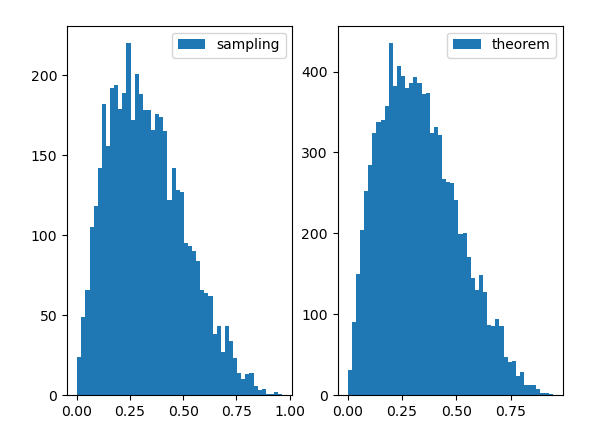
\includegraphics[width=0.5\textwidth]{1.png}
    \caption{Beta(2,4)}
    \end{figure} 


\end{enumerate}
\begin{enumerate}[(b)]
    \item
    From the figure shown as follow, histogram of sampling and theoretical PDF are basically the same.\\
    And in theory, (1)$Z\sim N(0,1)$\\
    (2)$X=\left\lvert Z\right\rvert $, then we can use exponential distribution to simulate it. And if we obtain x, then $z=x$ with 0.5 probability, and $z=-x$ with 0.5 probability.\\
    (3)$X=\left\lvert Z\right\rvert $, $f_X(x)=\frac{2}{\sqrt{2\pi}}e^{-\frac{1}{2}x^2}$, $0<x<\infty$.\\
    Then choose $g\sim Expo(1)$, $g(x)=e^{-x}$, $0<x<\infty$.\\
    Now $\frac{f(x)}{g(x)}=\sqrt{\frac{2}{\pi}}e^{-\frac{1}{2}x^2+x}$. And $c>=sup_x\frac{f(x)}{g(x)}$.\\
    And then we can have when $x=1$, we can get the correct $c=\sqrt{\frac{2e}{\pi}}$.\\
    Then we can have $\frac{f(x)}{g(x)c}=e^{-\frac{1}{2}(x-1)^2}$.\\
    So this derivation vertify and support the correctness of following modeling process. 
    \begin{figure}[htbp]
        \centering
        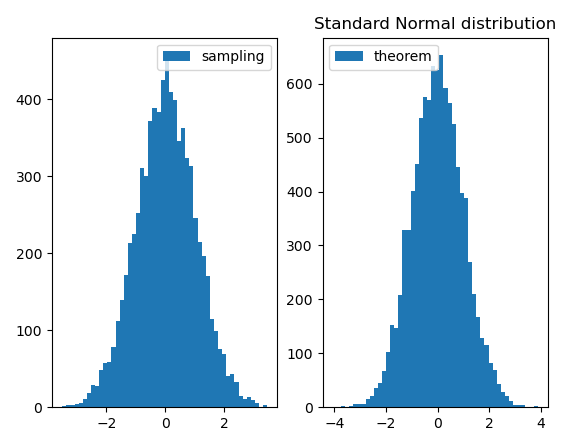
\includegraphics[width=0.5\textwidth]{2.png}
        \caption{Normal(0,1)}
        \end{figure} 
\end{enumerate}
\begin{enumerate}[(c)]
    \item
    The pros of the Acceptance-Rejection Method are that it is simple to implement and can be used to generate random variables from any distribution. The cons are that it can be computationally expensive and may not be efficient for generating random variables from distributions with complicated shapes.\\

    The pros of the Box-Muller Method are that it is simple to implement and computationally efficient. The cons are that it can only be used to generate random variables from the standard Normal distribution.\\
\end{enumerate}
\begin{enumerate}[(d)]
    \item
    c=6.167272764356622e-16(more details shown in the following code(4))
\end{enumerate}

\begin{verbatim}
    import random
    import math
    import matplotlib.pyplot as plt
    import numpy as np
    ##(1)
    ##because the process is calculated in class, so we directly use it
    ##c_beta=135/64, and f(Y)/c*g(Y)=(256/27)*Y(1-Y)^3
    accepted_X=[]
    x = np.linspace(0,1,1000)
    for i in range(0,10000):
        U=np.random.uniform(0,1)
        Y=np.random.uniform(0,1)
        FY=(256*Y*(1-Y)**3)/27
        if(U<=FY):
            X=Y
            accepted_X.append(X)
    plt.figure(1)
    plt.subplot(1,2,1)
    plt.hist(accepted_X,bins=50,label='sampling')
    plt.legend()
    ##theoretical
    plt.subplot(1,2,2)
    theorem_pdf_beta=np.random.beta(2,4,10000)
    plt.hist(theorem_pdf_beta,bins=50,label='theorem')
    plt.legend()
    plt.title("Beta distribution")
    plt.show()
    ##(2)
    accepted_Z=[]
    x = np.linspace(-3,3,1000)
    for i in range(0,10000):
        U=np.random.uniform(0,1)
        U_1=np.random.uniform(0,1)
        Y=np.random.exponential(1)##e^{-x}
        FY=np.exp(-0.5*(Y-1)**2)
        if(U<=FY):
            X=Y
            if(U_1<=0.5 and U_1>=0):
                Z=X
            elif(U_1>0.5 and U_1<=1):
                Z=-X
            accepted_Z.append(Z)
    plt.figure(2)
    plt.subplot(1,2,1)
    plt.hist(accepted_Z,bins=50,label='sampling')
    plt.legend()
    ##theoretical
    plt.subplot(1,2,2)
    theorem_pdf_beta=np.random.normal(0,1,10000)
    plt.hist(theorem_pdf_beta,bins=50,label='theorem')
    plt.legend()
    plt.title("Standard Normal distribution")
    plt.show()
    ##(4)
    # Define the function f(Y) = I(Y > 8)
    c=0
    for i in range(0,100000):
        Y=np.random.normal(8,1)
        f_1=np.exp(-Y**2/2)/np.sqrt(2*np.pi)
        f_2=np.exp(-(Y-8)**2/2)/np.sqrt(2*np.pi)
        if(Y>8):
            c+=f_1/f_2
        elif(Y<=8):
            c+=0
    c = c/100000
    print(c)
    
\end{verbatim}
\end{homeworkProblem}    
\end{document}
